\documentclass[conference]{IEEEtran}
\IEEEoverridecommandlockouts
% The preceding line is only needed to identify funding in the first footnote. If that is unneeded, please comment it out.
\usepackage{cite}
\usepackage{amsmath,amssymb,amsfonts}
\usepackage{algorithmic}
\usepackage{graphicx}
\usepackage{textcomp}
\usepackage{xcolor}
\usepackage{listings}
\usepackage{pgfplots}
\usepackage{float}
\usepackage{booktabs}
\pgfplotsset{compat=1.18}

\def\BibTeX{{\rm B\kern-.05em{\sc i\kern-.025em b}\kern-.08em
    T\kern-.1667em\lower.7ex\hbox{E}\kern-.125emX}}

\lstdefinestyle{mystyle}{
    basicstyle=\ttfamily\footnotesize,
    breakatwhitespace=false,         
    breaklines=true,                 
    captionpos=b,                    
    keepspaces=true,                                                       
    showspaces=false,                
    showstringspaces=false,
    showtabs=false,                  
    tabsize=2,
    frame=single,
    rulecolor=\color{black}
}

\lstset{style=mystyle}

\begin{document}

\title{Minimize Hand Displacement in a Song: Project 2 - Brute Force and Dynamic Programming}


\author{\IEEEauthorblockN{1\textsuperscript{st} Esteban Murillo}
\IEEEauthorblockA{\textit{Department of Computer Science} \\
\textit{Texas Tech University}\\
Lubbock, TX \\
estmuril@ttu.edu}
\and
\IEEEauthorblockN{2\textsuperscript{nd} Daniel Marin}
\IEEEauthorblockA{\textit{Department of Computer Science} \\
\textit{Texas Tech University}\\
Lubbock, TX \\
danimari@ttu.edu}
}

\maketitle

\begin{abstract}
This paper presents an algorithmic solution to optimize guitar chord transitions in musical sequences. We developed algorithms using both brute force and dynamic programming approaches to minimize left-hand displacement during chord changes. The system takes as input a sequence of chords in standard notation and a specification file containing multiple fingering positions for each chord. Our solution analyzes various possible chord positions and determines the optimal combination that minimizes the total hand movement throughout the song. The algorithms consider factors such as fret positions, string usage, and transitional distances between successive chord shapes. The results look to the difference and analyse the efficiency of the brute-force and dynamic programming approaches, based on the principal of demonstrating an effective method for reducing physical strain and improving playability in guitar performances through computational optimization.
\end{abstract}

\begin{IEEEkeywords}
dynamic programming, optimization algorithms, guitar chord transitions, musical computing, computational musicology, fingering optimization, performance automation
\end{IEEEkeywords}

\section{Introduction}
The optimization of musical performance through computational methods has become increasingly relevant in modern music technology. In this paper, we address a specific challenge in guitar playing: minimizing the left-hand movement during chord transitions.

When playing guitar, the positioning of the left hand on the fretboard significantly impacts both the physical effort required and the smoothness of the performance. A single chord can often be played in multiple positions on the fretboard, and the choice of these positions directly affects the distance the hand must travel when transitioning between chords. For instance, a C major chord can be played in several configurations, each requiring different finger placements and fret positions.

The challenge lies in determining the optimal sequence of chord positions that minimizes the total hand movement throughout an entire song. This optimization must consider various factors, such as: multiple valid fingering positions for each chord, the physical distance between successive chord positions, the practical playability of the chosen sequences, and the specific requirements of open strings and unused string in chord formations.

To solve this problem, we developed two distinct algorithmic approaches. The first utilizes a brute force method, examining all possible combinations of chord positions to find the global optimum. The second employs dynamic programming techniques to efficiently compute the optimal solution by breaking down the problem into smaller subproblems and avoiding redundant calculations.

Our solution takes two inputs: a sequence of chords in standard musical notation (e.g., C, Am, Dm, G7) and a specification dictionary that details the various possible fingering positions for each chord. The dictionary uses a numerical representation system where each chord is defined by a sequence of numbers representing the fret positions for each string, with special notation for open strings (0) and unused strings.

\section{Methodology}
The Methodology of this project, is based on explaining the problem definition, each solution, and the comparisons between both. We also look to solve the following problem:
\newline
\indent``Polynizer has hired the excellent students of CS-3364 to create an algorithm that allows to find the optimal way to play the chords that the application infers, on the guitar. Specifically, we want to minimize the amount of movement made by the left hand. The algorithm takes as input the list of chords of a song in standard notation (e.g., C, Am, Dm, G7, and C) and a file specifying different ways to play each chord, and should print on the screen how to play each chord in order to minimize the total movement of the hand over the song.''\footnote[1]{Problem Definition stated in the project definition document by Arturo Camacho.}
\subsection{Problem Outline}
The algorithm we are looking to develop processes a song's chord sequence in standard notation (e.g., C, Am, Dm, G7) alongside a file detailing various fingerings for each chord, with the end goal of outputting the optimal sequence of chord fingerings that minimize the total hand movement throughout the song. Before understanding how the algorithm's solve this problem we first need to understand how solutions and inputs look like.
\newline 
\indent Both algorithms take in the same parameters. These arguments are as follows: 

\textbf{Chord List}: that represents the sequence of $n$ chords in a song. This is what the user writes in `.txt' file. It has the expected format of a list/set of type, \[ C = \{c_1, c_2, c_3, \ldots, c_n\} \] where the \(c_i\) element in the list represents the \(i^{th}\) chord of the song. 

\textbf{Chord Dict}: a helper dictionary that contains all possible fingerings for each chord instance; considering their base frets. Thus providing a maaping from to fingerings available.

\indent These inputs remain consistent to both the brute-force search and the dynamic programming solution. Also, understanding the format of the inputs is required for comprehending the algorithms. Both algorithms return the same outputs, to answer/solve the overall problem the user has. The outputs are: optimal solution, optimal vector, and optimal sequence.

\textbf{Optimal solution} represents the minimum hand displacement calculated for the list of chords being displaced. This output are in units of `frets displaced'.

\textbf{Optimal vector} represents the vector \[ \sigma = \{\sigma_1, \sigma_2, \sigma_2, \ldots, \sigma_n\} \] where the \(\sigma_i\) element in this vector represents the fingering to be played in place of the \(i^{th}\) chord of the song. 
Where \( \sigma_i \in [0, K_i - 1] \), and \(K_i\) \footnote{A \(c_i\) with 3 fingerings has possible values \( \sigma_i \in [0, K_i - 1]\); where $0$ stands for the $1^{st}$ fingering in the .csv file for the chord, $1$ stands for the $2^{nd}$, and $2$ stands for the $3^{rd}$ fingering.} 
is the number of possible fingerings for the \(i^{th}\) chord. \footnote{Values range from \( [0, K_i - 1] \) due to enumerates in the program.}

\textbf{Optimal Sequence} represents the optimal vector as actual fingerings, it was used to debug the program.

\indent The outputs represent the solution towards the problem that we look to solve. They provide the how and the value of the solution to the problem. Understanding the inputs and outputs as a black box (the algorithms), we need to look at some overlapping functions that are used to calculate displacement based on what the professor stated in the project definition document.
\subsection{Helper Functions}
The functions in this section look to provide a simple method to calculate the overall displacement between two chords. 
\begin{figure}[H]
\begin{lstlisting}[language=Python]
def calculate_average_fret(x):
    accum : int = 0
    frets : int = 0
    for fret in x:
        if fret is not None:
            accum += fret
            frets += 1
    return accum / frets if frets > 0 else 0.0
def calculate_movement_displacement(a, b):
    average_fret_a = calculate_average_fret(a)
    average_fret_b = calculate_average_fret(b)
    return (average_fret_a - average_fret_b)**2    
\end{lstlisting}
\caption{Uncommented functions in charge of calculating displacement of between fingerings, used in this project. Based, on program specifications in project definition document.}
\label{fig:DisplacementFunctions}
\end{figure}
The functions in Figure \ref{fig:DisplacementFunctions} are used to measure the displacement of the left hand on a guitar when transitioning between chord positions. The \lstinline|calculate_average_fret(x)| function calculates the centroid of a chord position by adding the fret numbers of all strings where the chord is fingering, and dividing it by the number of strings used by the fingering. For example: 
\[ \text{Centroid}_a  = \frac{0+2+2+2+0}{5} = 1.2 \] 
\[ \text{Centroid}_b = \frac{3+5+5+5+3}{5} = 4.2 \]
\indent Where \( \text{Centroid}_a \) represents chord A and \(\text{Centroid}_b \) represents chord C. 
\newline 
\indent The \lstinline|calculate_movement_displacement(a, b)| looks to calculate the displacement between two chords by calculating the following:
\[
\text{Displacement} = (\text{Centroid}_a + \text{Centroid}_b)^2
\]
\indent These function help the algorithm's minimize the processes being called, by centralizing them. With this understood, we may begin explaining the brute-force search algorithm that solves this problem.
\subsection{Brute-force Search}
Brute-force search is a straightforward and exhaustive problem-solving technique that systematically explores all possible solutions to a problem to identify the optimal one. It works by generating every potential candidate in the solution space, evaluating each against a given objective or constraint, and selecting the best match. While simple to implement and guaranteed to find the correct solution, brute-force search is often computationally expensive, as the number of possibilities grows exponentially with the size of the input. 
\subsubsection{Algorithm Design}
The algorithm designed for this project, regarding brute-force search, used exhaustive exploration of all possible sequences of fingerings from the chord list. 
There are various considerations, that should be looked at before evaluating the implementation of the algorithm: vector representation, its possible values, the space and its size.
\newline 
\noindent The vector has the same representation from the Problem Outline, that being: \[ \sigma = \{\sigma_1, \sigma_2, \sigma_3, \ldots, \sigma_n\}. \] 
\indent Where \(\sigma_i \in [0, K_i - 1]\), and where \( K_i \) represents the number of possible fingerings of the $i^{th}$ chord in the song. If the resultant vector represents the solution, the vector space can be expressed as:
\[ S = \{0, \frac{\sum_{i=1}^{n}K_i - 1}{n} \}^{n}. \]
\indent This setup of the vector space leads it to be upper bounded by \( S = \{0,1,2\}^{n} \), considering that the worst case scenario is a song composed of chords with $3$ fingerings available. The vector space size is:
\[ |S| = 3^{n}. \].
\indent However, considering that there is a constraint where we should only allow chord fingerings that have base fret position of 7 or less, the space $S$ is further reduced to a subset $S'$ defined as:
\[ S' = \{\sigma \in S \mid \text{minimum fret position of \( F(C_{\sigma_i}) \)} \leq 7, \forall(i)\}. \]
\indent This leads to a reduction in the vector space by an incalculable amount but in theory it should decrease or maintain the same.
\[ |S'| \leq |S|. \]

\subsubsection{Asymptotic Time Complexity}
This algorithm has a time complexity of \(\Theta(3^{n})\) in the worst-case scenario, implying that this algorithm takes exponential time and is fairly inefficient for medium to large input sizes.  

\subsubsection{Code Implementation}
The brute force algorithm is implemented through several key components:

\begin{figure}[H]
\begin{lstlisting}[language=Python]
def minimum_movement_brute_force(chord_list, chord_dict):
    chord_fingerings = []
    for chord in chord_list:
        if chord in chord_dict:
            fingerings = []
            fingerings.append(chord_dict[chord]['Finger A'])
            if 'Finger B' in chord_dict[chord]:
                fingerings.append(chord_dict[chord]['Finger B'])
            if 'Finger C' in chord_dict[chord]:
                fingerings.append(chord_dict[chord]['Finger C'])
            chord_fingerings.append(fingerings)
\end{lstlisting}
\caption{First part of the brute force implementation: gathering possible fingerings}
\label{fig:BruteForceGather}
\end{figure}

The first part of the implementation (Figure \ref{fig:BruteForceGather}) focuses on gathering all possible fingerings for each chord in the sequence. The algorithm creates a list of available fingerings for each chord position, supporting up to three different fingering options (A, B, and C) per chord. 

\begin{figure}[H]
\begin{lstlisting}[language=Python]
    for idx_combination in product(*[range(len(f)) for f in chord_fingerings]):
        sequence = [chord_fingerings[i][idx_combination[i]] 
                   for i in range(len(chord_list))]
        
        cost = total_movement_cost(sequence)
        
        if cost < min_cost:
            min_cost = cost
            min_cost_sequence = sequence
            min_cost_indices = list(idx_combination)
\end{lstlisting}
\caption{Core loop of the brute force implementation: evaluating all combinations}
\label{fig:BruteForceCore}
\end{figure}

The core of the algorithm (Figure \ref{fig:BruteForceCore}) systematically evaluates every possible combination of fingerings. It uses Python's \lstinline{itertools.product} to generate all possible combinations of fingering indices for the song. 

For each combination: create a sequence of actual fingerings using the current combination, calculate the total movement cost for this sequence, and updates the optimal solution if a lower cost is found.

\begin{figure}[H]
\begin{lstlisting}[language=Python]
def total_movement_cost(sequence):
    cost = 0
    for i in range(1, len(sequence)):
        cost += calculate_movement_displacement(sequence[i-1], sequence[i])
    return cost 
\end{lstlisting}
\caption{Helper function for calculating total movement cost}
\label{fig:BruteForceCost}
\end{figure}

The movement cost calculation (Figure \ref{fig:BruteForceCost}) iterates through the sequence of chords, summing up the displacement cost between consecutive chord positions. The first chord position serves as the starting point and doesn't contribute to the total cost.\footnote{The resultant minimum cost is returned as the square root of the calculated cost to normalize the value into frets displaced.}

The bounded version of the algorithm adds an additional constraint check:
\begin{lstlisting}[language=Python]
    if any(min(fret for fret in fingering if fret is not None) > 7 
           for fingering in sequence):
        continue
\end{lstlisting}

This optimization ensures that only fingerings within the first seven frets are considered, which both reduces the search space and produces more practical solutions for guitar players.

\subsection{Dynamic Programming}
Dynamic Programming (DP) is an algorithmic paradigm that solves complex problems by breaking them down into simpler subproblems. For our chord transition optimization, it is applicable because: each chord transition decision affects future transitions (overlapping subproblems), the optimal solution builds upon optimal solutions to smaller sequences (optimal substructure), and many chord transition patterns are evaluated multiple times (memoization opportunity).

By leveraging on these characteristics, we can systematically model and solve the problem. A key step in this process if defining the \textbf{Oracle} - the table that encapsulates the state space and transition rules of the problem.

\subsubsection{Oracle Definition}
The Oracle is defined as: \(C_{i,j}\) is equal as the minimum total movement cost from the first chord to the \(i^{th}\) chord; assuming the \(i^{th}\) is being played with the \(j^{th}\) fingering. Where \(i\) represents the index of the current chord in the list, and \(j\) represents the index of the chosen fingering of the current chord. 
It is important to state that a fingering \(f\) for any chord is only considered and used in the Oracle if:
\[ \min(\{\forall x \in f \mid x \neq \text{None}\}) \leq 7. \]

Considering the setup we may begin to demonstrate the logic for each of the steps that fill up the Oracle and provide us with the solution. 

\subsubsection{Dynamic Programming Steps}
To comprehend the steps defined we must understand the Base Step, the Recursive Step and the Goal. The creation of the oracle and the retrieval of a solution is provided as follows:

The \textbf{Base Step} is \[ C_{1,f} = 0 \text{, \(\forall f\) where \(f\) is a fingering of chord \(c_1\) }, \] since the initial chord doesn't initialize a cost to the problem. The \textbf{Recursive Step} is \[ C_{i,f} = \min_{p \in [1, K_{i-1}]}(C_{i-1, p} + cost(a, b)), \] where \(a\) is the \(p^{th}\) fingering of chord \(c_{i-1}\) and \(b\) is the \(f^{th}\) fingering of chord \(c_i\), such that \(cost(a,b)\) is the cost of the displacement between \(a\) and \(b\). Lastly, the \textbf{Goal} is \[ \min_{p \in [1, K_{n}]}(C_{n, p}), \] where we select the minimum cost of playing the final chord, based on playing it with \(p^{th}\) fingering.

It is important to understand that indices are (for practical purposes) are being displayed from 1 to $n$ to better understand the math behind the Oracle. In practice these indices are accessed with an offset of $-1$ ranging from 0 to $n-1$. Slight alterations take place to comply with the programming language, but the logic behind the dynamic programming has the same format.

Utilizing the Oracle definition and the steps defined above, the implementation will be discussed in the following subsection.

\subsubsection{Algorithm Implementation}
The implementation consists of four main components: initialization, oracle construction, solution reconstruction and cost normalization.

The \textbf{Initialization} is the process of collecting valid fingerings for each chord from the chord dictionary, creating the oracle and solution dictionaries for each chord position, and setting the base costs for the first chord's valid fingerings.

The \textbf{Oracle Construction} is generated using the Recursive Step in the program as follows:
\begin{lstlisting}[language=Python]
    # Fill the Oracle
    for i in range(1, n):
        for f, fingering in enumerate(chord_fingerings[i]):
            if not is_valid_fingering(fingering):
                continue
            Oracle[i][f] = float('inf')
            for f_prev, prev_fingering in enumerate(chord_fingerings[i - 1]):
                if not is_valid_fingering(prev_fingering):
                    continue
                cost = Oracle[i - 1][f_prev] + calculate_movement_displacement(prev_fingering, fingering)
                if cost < Oracle[i][f]:
                    Oracle[i][f] = cost
                    Solution[i][f] = f_prev
\end{lstlisting}

The \textbf{Solution Construction} looks to identify the minimum cost fingerings for final chord, traces back through the solution dictionary to build the optimal sequence; with the end result of returning the outputs of this algorithm properly. 

Lastly, the \textbf{Cost Normalization} is simply the normalization of the minimul cost from `frets displaced$^{2}$' to `frets displaced'.

\subsubsection{Time Complexity}
The algorithm discussed above achieves a time complexity of \[ \Theta(nK^2) \] 
where $n$ is the number of chords in the sequence, and $K$ is the maximum number of valid fingerings for each chord. We must comprehend that $K$ in the worst-case scenario $K$ is a constant value of $3$ the time complexity is of \(\Theta(n \times 9) \) which means that this algorithm takes linear time to execute.

This is significantly more efficient than the brute-force search approach, with a time complexity of \(\Theta(3^n)\) as it: eliminates redundant calculations through memoization, prunes invalid fingering combinations early, and builds the solution incrementally using optimal substructure.


\subsubsection{Code Implementation}
The dynamic programming algorithm is implemented through several key components. It uses a \textbf{Helper Functions} to facilitate the validation of fingerings:
\begin{lstlisting}[language=Python]
def is_valid_fingering(fingering):
    valid_frets = [fret for fret in fingering if fret is not None]
    if not valid_frets:
        return False
    return min(valid_frets) <= 7
\end{lstlisting}

The validation function ensures that the algorithm only considers frets that are actually used (not None), returns false if no valid frets exist, enforces the constraint that minimum fret position must be \(\leq 7\).

The creation of fingering collections is performed by:
\newpage
\begin{lstlisting}[language=Python]
    chord_fingerings = []
    for chord in chord_list:
        if chord in chord_dict:
            fingerings = []
            for key in ['Finger A', 'Finger B', 'Finger C']:
                if key in chord_dict[chord]:
                    fingering = chord_dict[chord][key]
                    fingerings.append(fingering)
\end{lstlisting}

This initialization phase looks to process each chord in the input sequence while collecting up to three valid fingerings (A, B, C) per chord in the dictionary.
Before delving into the core logic, we need to fill up the base step. This process is performed by the following logic:
\begin{lstlisting}[language=Python]
    n = len(chord_list)
    Oracle = [{} for _ in range(n)]  # Each entry is a dictionary
    Solution = [{} for _ in range(n)]  # Tracks previous indices
    
    # Initialize base case
    for f, fingering in enumerate(chord_fingerings[0]):
        if is_valid_fingering(fingering):
            Oracle[0][f] = 0
\end{lstlisting}
This setup initalizes the two dictionaries for the Oracle and the Solution, and also begins the Oracle with the aforementioned Base Step. Considering the initial setup, the core dynamic programming logic of this algorithm implementation is as follows:
\begin{lstlisting}[language=Python]
    for i in range(1, n):
        for f, fingering in enumerate(chord_fingerings[i]):
            if not is_valid_fingering(fingering):
                continue
            Oracle[i][f] = float('inf')
            for f_prev, prev_fingering in enumerate(chord_fingerings[i - 1]):
                if not is_valid_fingering(prev_fingering):
                    continue
                cost = Oracle[i - 1][f_prev] + calculate_movement_displacement(
                    prev_fingering, fingering)
                if cost < Oracle[i][f]:
                    Oracle[i][f] = cost
                    Solution[i][f] = f_prev
\end{lstlisting}
This main algorithm iterates through each chord position for each valid current fingering, while considering all valid previous fingerings and filling up the oracle and the solution with the minimum cost and the solution vector in the process. With this, the last part of the algorithm is to reconstruct the solution once the Oracle has been filled, this processs is done by: starting form the optimal final fingering, tracing back through the Solution dictionary, building both the fingering and the index sequence, and reversing the sequence to get the beginning to end traversal of the solution. This is done with the following algorithm:
\newpage
\begin{lstlisting}[language=Python]
sequence = []
indexes = []
f = min_cost_index
for i in range(n - 1, -1, -1):
    sequence.append(chord_fingerings[i][f])
    indexes.append(f)
    f = Solution[i].get(f, None)
sequence.reverse()
indexes.reverse()
\end{lstlisting}

The implementation uses dictionaries instead of traditional arrays to efficiently handle varying numbers of valid fingerings per chord. The final cost is normalized using square root to maintain consistency with the problem's distance metric.



\subsection{Greedy Approach}
A greedy algorithm was not implemented for this problem because a greedy approach cannot guarantee an optimal solution for chord sequence optimization. Here's why:

A greedy algorithm would make locally optimal choices at each step, selecting the chord fingering that minimizes movement from the current position. However, these local choices do not necessarily lead to a globally optimal solution. Let's look at the following example:

For a sequence ``C-Am-G'' a greedy approach might choose the closest fingering of Am to the inital C chord position, and then closest G fingering to the Am position. This could result in a larger total movement than choosing a slighlty ``worse'' initial transition that enables a much better final transition.

The problem requires considering the entire sequence of transitions to find the true optimal solution, which is why we implemented: brute-force search, since it guarantees optimality by checking all possibilities; and dynamic programming approach, efficiently finds the optimal sequence by considering all possible combinations systematically.

Therefore, this project focuses on the brute force and dynamic programming solutions as they are capable of finding the globally optimal solution to the chord sequence optimization problem.

\section{Tests}
To evaluate the performance and effectiveness of both algorithms, we conducted tests using three musical pieces provided by the professor: Luis Miguel - El Dia Que Me Quieras, Halsey - Graveyard, and Toto - Hold The Line. 

\subsection{Test Setup}
Each algorithm was tested with different chord sequence lengths to analyze their scalability and performance characteristics:

\subsubsection{Brute Force Test Cases}
Brute-force search was tested utilizing increments of 4 up to 20 chords in a chord sequence, an example of this sequence would be: 4, 8, 12, 16 and 20 chords in a sequence.  

\subsubsection{Dynamic Programming Test Cases}
Dynamic Programming being a better performing algorithm was tested utilizing increments of 40 starting at 20, up to the maximum input size of a song; and also by utilizing the increments defined for the Brute-Force Search. Such as, the following test for Toto - Hold The Line: 4, 8, 12, 16, 20, 60, 100, 140, 180 and 206 chords in a sequence.

\section{Results}
Before delving into the discussion of results and conclusions, it is important to state that both the brute-force search and the dynamic programming algorithm's have been tested and compared to the results provided by Dr. Camacho as a proof for proper behavior. For all test cases in this section, the minimum cost is the same as the one provided by the professor. 

\subsection{Analysis of Toto's - Hold The Line}
\begin{table}[H]
    \centering 
    \caption{Brute-Force Search Execution Times - Hold The Line}
    \renewcommand{\arraystretch}{1.2} % Increases row height for readability
    \setlength{\tabcolsep}{3pt} % Adjusts padding between columns
    \begin{tabular}{r r}
        \toprule
        \textbf{Input Size ($n$)} & \textbf{Execution Time ($s$)} \\
        \midrule 
        4 & 0.000231 \\
        8 & 0.002293 \\
        12 & 0.106462 \\
        16 & 1.525553 \\ 
        20 & 27.776092 \\
        \bottomrule
    \end{tabular}
\end{table}

\begin{table}[H]
    \centering
    \caption{Dynamic Programming Execution Times - Hold The Line}
    \renewcommand{\arraystretch}{1.2} % Increases row height for readability
    \setlength{\tabcolsep}{3pt} % Adjusts padding between columns
    \begin{tabular}{r r}
        \toprule 
        \textbf{Input Size ($n$)} & \textbf{Execution Time ($s$)} \\
        \midrule 
        4 & 0.000107 \\
        8 & 0.000142 \\
        12 & 0.000177 \\
        16 & 0.000221 \\
        20 & 0.000283 \\
        60 & 0.000652 \\
        100 & 0.000964 \\
        140 & 0.001265 \\
        180 & 0.001642 \\
        206 & 0.001821 \\
        \bottomrule
    \end{tabular}
\end{table}

Considering the results in both of the tables in here, a plot may be developed as follows, to indicate correlations between the input size and the execution time for these two algorithms.

\begin{figure}[H]
    \centering
    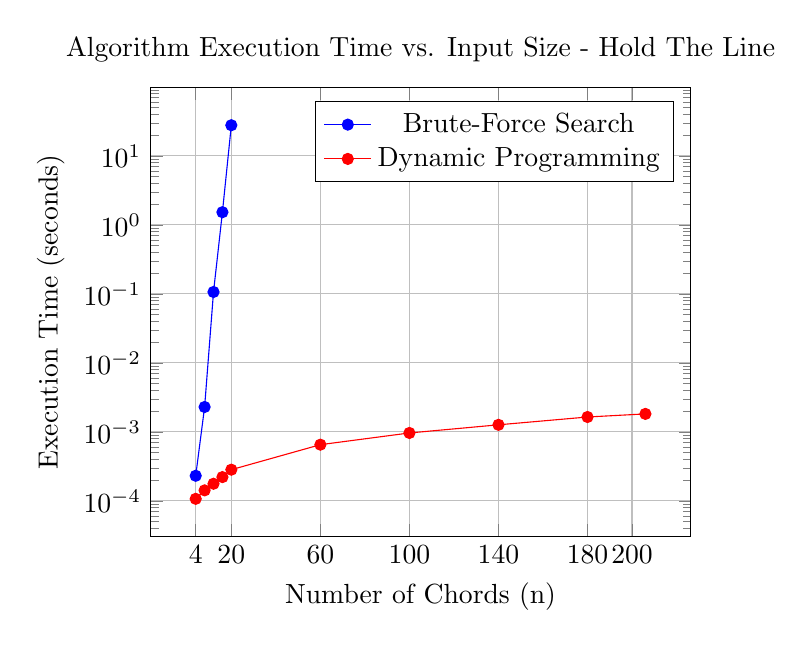
\begin{tikzpicture}
        \begin{axis}[
            xlabel={Number of Chords (n)},
            ylabel={Execution Time (seconds)},
            xtick={4,20,60,100,140,180,200},
            title={Algorithm Execution Time vs. Input Size - Hold The Line},
            grid=major,
            legend pos=north east,
            legend entries={Brute-Force Search, Dynamic Programming},
            ymode=log
        ]
        % Brute-Force Search data
        \addplot[color=blue, mark=*] coordinates {
            (4, 0.000231) (8, 0.002293) (12, 0.106462) (16, 1.525553) (20, 27.776092)
        }; 
        % Dynamic Programming data
        \addplot[color=red, mark=*] coordinates {
            (4, 0.000107) (8, 0.000142) (12, 0.000177) (16, 0.000221) (20, 0.000283) 
            (60, 0.000652) (100, 0.000964) (140, 0.001265) (180, 0.001642) (206, 0.001821)
        };
        \end{axis}
    \end{tikzpicture}
    \caption{Execution Time Comparison Between Brute-Force Search and Dynamic Programming - Hold The Line}
    \label{fig:execution-time}
\end{figure}

\textbf{Results Discussion}: The plot in Figure \ref{fig:execution-time} demonstrates consistency with the execution times for Brute-Force Search and the Dynamic Programming respective algorithms. 

Were Brute-Force Search is clearly shown to have an exponential growth pattern, with execution times increasing as the number of chords increases. This aligns with the algorithm's theoretical time complexity of $\Theta(3^{n})$, where $n$ is the input size. The steep curve between 12 and 16.

Meanwhile, Dynamic Programming Contains a slight linear increase as the input size increases maintaining consistency between the theoretical time complexity of this algorithm of $\Theta(n)$. 

\subsection{Analysis Luis Miguel's - El Dia Que Me Quieras}
\begin{table}[H]
    \centering 
    \caption{Brute-Force Search Execution Times - El Dia Que Me Quieras}
    \renewcommand{\arraystretch}{1.2} % Increases row height for readability
    \setlength{\tabcolsep}{3pt} % Adjusts padding between columns
    \begin{tabular}{r r}
        \toprule 
        \textbf{Input Size ($n$)} & \textbf{Execution Time ($s$)} \\
        \midrule
        4 & 0.000349 \\
        8 & 0.008179 \\
        12 & 0.105452 \\
        16 & 0.806655 \\ 
        20 & 46.038268 \\
        \bottomrule
    \end{tabular}
\end{table}
\begin{table}[H]
    \centering
    \caption{Dynamic Programming Execution Times - El Dia Que Me Quieras}
    \renewcommand{\arraystretch}{1.2} % Increases row height for readability
    \setlength{\tabcolsep}{3pt} % Adjusts padding between columns
    \begin{tabular}{r r}
        \toprule 
        \textbf{Input Size ($n$)} & \textbf{Execution Time ($s$)} \\
        \midrule 
        4 & 0.000080 \\
        8 & 0.000121 \\
        12 & 0.000152 \\
        16 & 0.000176 \\
        20 & 0.000233 \\
        60 & 0.000530 \\
        100 & 0.000909 \\
        140 & 0.001237 \\
        147 & 0.001311 \\
        \bottomrule
    \end{tabular}
\end{table}
\begin{figure}[H]
    \centering
    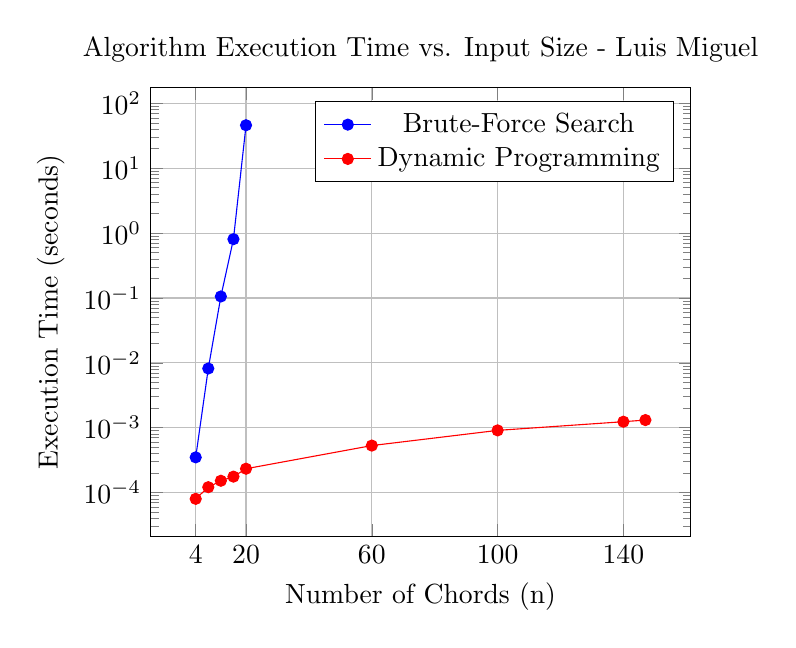
\begin{tikzpicture}
        \begin{axis}[
            xlabel={Number of Chords (n)},
            ylabel={Execution Time (seconds)},
            xtick={4,20,60,100,140},
            title={Algorithm Execution Time vs. Input Size 
            - Luis Miguel},
            grid=major,
            legend pos=north east,
            legend entries={Brute-Force Search, Dynamic Programming},
            ymode=log
        ]
        % Brute-Force Search data
        \addplot[color=blue, mark=*] coordinates {
            (4, 0.000349) (8, 0.008179) (12, 0.105452) (16, 0.806655) (20, 46.038268)
        }; 
        % Dynamic Programming data
        \addplot[color=red, mark=*] coordinates {
            (4, 0.000080) (8, 0.000121) (12, 0.000152) (16, 0.000176) (20, 0.000233) 
            (60, 0.000530) (100, 0.000909) (140, 0.001237) (147, 0.001311)
        };
        \end{axis}
    \end{tikzpicture}
    \caption{Execution Time Comparison Between Brute-Force Search and Dynamic Programming - El Dia Que Me Quieras}
    \label{fig:execution-time-2}
\end{figure}

\textbf{Results Discussion}: Again, the results remain consistent. The execution time results demonstrate the exponential nature of the brute force algorithm (Blue line). 
The graph clearly shows the exponential growth pattern, with execution time increasing dramatically as the number of chords increases. This aligns with the algorithm's theoretical time complexity of \(\Theta(3^n)\), where n is the number of chords. The steep curve between 10 and 15 chords particularly highlights why brute force becomes impractical for longer sequences.
In contrast, the dynamic programming solution (Red line) demonstrates remarkably consistent performance.

For sequences of sixty chords, the execution time was merely 0.000530s. When increased to one hundred chords, the algorithm maintained its efficiency at 0.000909s. Even at one hundred forty chords, it demonstrated consistent performance at 0.001237s.

The dynamic programming results showcase several key advantages. In terms of scalability, the algorithm maintains near-constant execution times even as the input size triples from 40 to 120 chords. Its efficiency is particularly notable, as processing 120 chords takes approximately the same time as the brute force approach needs for just 5 chords. The consistency is demonstrated through slight variations in execution time (between 0.000977s and 0.001509s), showing stable performance regardless of input size. Finally, the practical applicability is evident in the algorithm's ability to handle large chord sequences in milliseconds, making it suitable for real-world applications.

These results validate the theoretical time complexity of \(\Theta(n \times K^2)\) for the dynamic programming solution, where n is the number of chords and K is the maximum number of fingerings per chord. The nearly flat line in the graph demonstrates how this polynomial-time complexity translates to practical performance benefits, especially when compared to the exponential growth of the brute force approach.

\subsection{Analysis of Halsey's - Graveyard}
\begin{table}[H]
    \centering 
    \caption{Brute-Force Search Execution Times - Graveyard}
    \renewcommand{\arraystretch}{1.2} % Increases row height for readability
    \setlength{\tabcolsep}{3pt} % Adjusts padding between columns
    \begin{tabular}{r r}
        \toprule 
        \textbf{Input Size ($n$)} & \textbf{Execution Time ($s$)} \\
        \midrule 
        4 & 0.000176 \\
        8 & 0.001854 \\
        12 & 0.033095\\
        16 & 0.202635 \\
        20 & 15.449490 \\
        \bottomrule
    \end{tabular}
\end{table}
\begin{table}[H]
    \centering
    \caption{Dynamic Programming Execution Times - Graveyard}
    \renewcommand{\arraystretch}{1.2} % Increases row height for readability
    \setlength{\tabcolsep}{3pt} % Adjusts padding between columns
    \begin{tabular}{r r}
        \toprule 
        \textbf{Input Size ($n$)} & \textbf{Execution Time ($s$)} \\
        \midrule 
        4 & 0.000076 \\ 
        8 & 0.000105 \\
        12 & 0.000141 \\
        16 & 0.000187 \\
        20 & 0.000208 \\
        60 & 0.000646 \\
        100 & 0.001207 \\
        128 & 0.001611 \\
        \bottomrule
    \end{tabular}
\end{table}
\begin{figure}[H]
    \centering
    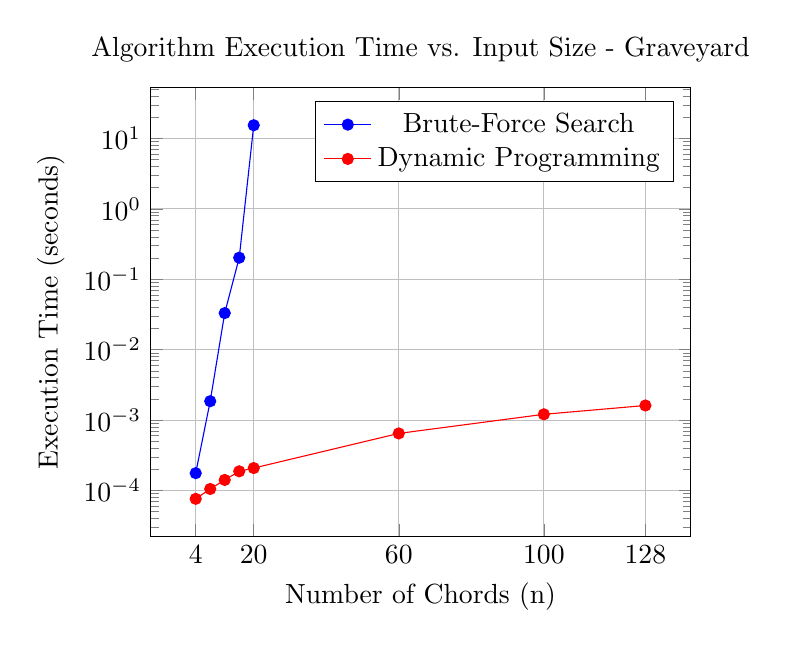
\begin{tikzpicture}
        \begin{axis}[
            xlabel={Number of Chords (n)},
            ylabel={Execution Time (seconds)},
            xtick={4,20,60,100,128},
            title={Algorithm Execution Time vs. Input Size - Graveyard},
            grid=major,
            legend pos=north east,
            legend entries={Brute-Force Search, Dynamic Programming},
            ymode=log
        ]
        % Brute-Force Search data
        \addplot[color=blue, mark=*] coordinates {
            (4, 0.000176) (8, 0.001854) (12, 0.033095) (16, 0.202635) (20, 15.449490)
        }; 
        % Dynamic Programming data
        \addplot[color=red, mark=*] coordinates {
            (4, 0.000076) (8, 0.000105) (12, 0.000141) (16, 0.000187) (20, 0.000208) 
            (60, 0.000646) (100, 0.001207) (128, 0.001611)
        };
        \end{axis}
    \end{tikzpicture}
    \caption{Execution Time Comparison Between Brute-Force Search and Dynamic Programming - Graveyard}
    \label{fig:execution-time-graveyard}
\end{figure}
\textbf{Analysis of Results}: The execution time results for the Halsey song demonstrate similar patterns to the previous analysis, where Brute Force displays inefficient exponential execution times. Meanwhile, dynamic programming produces linear and consistent results. 

It is important to note that results may vary significantly in some values due to number of possible each fingerings has. With this said let's begin our conclusive discussion.


\section{Conclusion}
The experimental results from the test cases (Toto, Luis Miguel and Halsey songs) provide clear evidence of the significant performance differences between brute-force search and dynamic programming approaches for the problem at hand.

\subsection{Performance Analysis}

The brute force approach demonstrates significant limitations in its performance. The algorithm exhibits clear exponential growth (\(\Theta(3^n)\)) in execution time, becoming impractical for sequences beyond 15-20 chords. This limitation is clearly demonstrated in our test results: for a sequence of 20 chords, the Luis Miguel test required 65.97 seconds to complete, while the Halsey test took 19.81 seconds for the same number of chords.
    
In contrast, the dynamic programming solution demonstrates remarkably consistent performance. The algorithm maintains consistent performance with its theoretical time complexity of \(\Theta(n \times K^2)\), processing sequences of 120 chords in approximately 0.001 seconds. It shows negligible variation in execution time across different songs and scales efficiently with increased input size, making it a far more practical solution for real-world applications.

\subsection{Practical Implications}
The test results demonstrate that while both algorithms find optimal solutions:

Dynamic programming is the clear choice for practical applications. It offers the ability to handle full-length songs efficiently, provides consistent performance across different musical styles, and delivers the necessary scalability for real-time applications.

The brute force approach, however, is only suitable for very short chord sequences (under 15 chords), educational purposes; demonstrating algorithmic concepts, and verification of dynamic programming results.

\subsection{Final Observations}
The implementation and testing of both algorithms reveal that the choice between brute force and dynamic programming for chord sequence optimization isn't merely about theoretical complexity—it has practical implications for usability. The dynamic programming solution achieves the project's goal of providing a practical tool for minimizing hand movement in guitar performances. The exponential growth of the brute-force search makes it unsuitable for real-world applications despite its conceptual simplicity. The consistent sub-millisecond performance of dynamic programming enables its use in interactive music applications.

This project demonstrates the importance of selecting appropriate algorithmic approaches for optimization problems in musical computing, where efficiency and scalability are crucial for practical applications.


% \begin{thebibliography}{00}

% \end{thebibliography}

\end{document}